\chapter{Numerical modelling of fluid–grain interactions}

\ifpdf
    \graphicspath{{Chapter5/figs/raster/}{Chapter5/figs/pdf/}{Chapter5/figs/}}
\else
    \graphicspath{{Chapter5/figs/vector/}{Chapter5/figs/}}
\fi


\section{Fluid simulation using lattice Boltzmann method}

Grain--fluid systems can be found in many scientific and engineering 
applications, such as suspensions, fluidised beds, sediment transport, and 
geo-mechanical problems. In general, the fundamental physical phenomena in 
these systems are not well understood mainly due to the intricate complexity of 
grain--fluid interactions and the lack of powerful analysis 
tools~\citep{Han2007b}. In addition to the interaction among soil grains, the 
motion of soil grains is mainly driven by gravity and the hydrodynamic force 
exerted by the fluid. The fluid flow pattern can be significantly 
affected by the presence of soil grains and this often results in a turbulent 
flow. Hence, the development of an effective numerical framework for modelling 
both the fluid flow patterns and the grain--fluid interactions is very 
challenging.

Development of a numerical framework depends crucially on the size of the soil 
grains relative to the domain/mesh size~\citep{Feng2007}. Traditionally, the 
Navier-Stokes equation is solved by a grid-based Computational Fluid Dynamics 
(CFD) method, such as the Finite Volume Method, FVM,~\citep{Capecelatro2013} or 
a mesh-free technique such as Smooth Particle Hydrodynamics
(SPH)~\citep{Sun2013}. 
The grid size in FVM or the smooth length in SPH for discretisation of 
the Navier-Stokes equation is at least an order of magnitude larger than the 
grain diameter~\citep{Xiong2014}. 

In situations where the average domain concentration phase is far from dilute, 
the computational effort is mostly devoted to the grain dynamics. The 
hydrodynamic forces on the soil grains are applied based on an empirical 
relation using the domain-averaged local porosity of the soil grains in the 
grid. As a result, developing a fast fluid hydrodynamics solver is unimportant 
for dense flows. However, most geo-mechanical problems involve complex 
interactions between the solid and the fluid phase. This requires accurate 
modelling of the fluid flow pattern. Additionally, geophysical problems, such 
as submarine landslides and debris flow have a relatively large simulation 
domain, which requires parallel computation. Implementing traditional 
grid-based CFD methods face great challenges on multi-processor 
systems~\citep{Xiong2014}. Although mesh-free approaches are free from the 
problem of parallel scalability, its modelling accuracy and speed are 
relatively low when compared to grid-based CFD methods. Therefore, an accurate, 
fast and a highly scalable scheme is required to model fluid - grain systems in 
geo-mechanics. 
 
The Navier-Stokes equation describes the motion of a non-turbulent Newtonian 
fluid. The equation is obtained by applying Newton's second law to the fluid 
motion, together with an assumption that the fluid stress is the sum of the 
viscous term, proportional to the gradient of the velocity, and the pressure 
term. Conventional CFD methods compute pertinent flow fields, such as velocity 
\textit{u} and pressure \textit{p}, by numerically solving the Navier-Stokes 
equation in space \textit{x} and time \textit{t}. Alternatively, the transport 
equation or the Boltzmann equation, which deals with a single particle 
distribution function $f(x,\xi,t)$ in phase space $(x,\xi)$ and time 
\textit{t}, can be used to solve various problems in fluid dynamics. 

The Lattice Boltzmann Method
(LBM)~\citep{He1997a,He1997b,Chen1998a,Mei2000,Han2007a,Zhou2012}
is an alternative approach to the classical Navier-Stokes solvers for fluid 
flows. LBM works on an equidistant grid of cells, called lattice cells, which 
interact only with their direct neighbours. In LBM, the discretisation of 
continuum equations is based on microscopic models and mesoscopic continuum 
theories. LBM is a special discretising scheme of the Boltzmann equation where 
the particle distribution functions (mass fractions) collide and propagate on a 
regular grid. The important aspect, however, is the \textit{discretisation of 
the velocity}, which means that the particle velocities are restricted to a 
predefined set of orientations.

The theoretical premises of the LB equation are that (1) hydrodynamics is 
insensitive to the details of microscopic physics, and (2) hydrodynamics can be 
preserved so long as the conservation laws and associated symmetries are 
respected in the microscopic and mesoscopic level. Therefore, the computational 
advantages of LBM are achieved by drastically reducing the particle velocity 
space $\xi$ to only a very few discrete points without seriously degrading the
hydrodynamics~\citep{Mei2000}. This is possible because LBM rigorously 
preserves the hydrodynamic moments of the distribution function, such as mass 
density and momentum fluxes, and the necessary 
symmetries~\citep{He1997a,He1997b}.
% The process of averaging the density and the momentum over some regions of 
%the space, i.e. coarse graining, produces some useful fluid simulation. 
LBM has evolved as a comprehensive fluid solver and its theoretical aspects 
link well with the conventional central finite difference 
scheme~\citep{Cook2004}.

\subsection{Formulation}

LBM is a `micro-particle' based numerical time-stepping procedure for the 
solution of incompressible fluid flows. Consider a 2D incompressible fluid flow 
with density $\rho$ and kinematic viscosity \textit{v}, in a rectangular domain 
\textit{\textbf{D}}. The fluid domain is divided into rectangular grids or 
lattices, with the same grid length \textit{`h'} in both \textit{x-} and 
\textit{y-}directions (see~\cref{fig:D2Q9}). 

\begin{figure}[htpb]
	\centering
	\includegraphics[width=0.95\textwidth]{D2Q9}
	\caption[The lattice Boltzmann discretisation and D2Q9 scheme]{The Lattice 
	Boltzmann discretisation and D2Q9 scheme: (a) a standard LB lattice and 
	histogram views of the discrete single particle distribution 
	function/direction-specific densities $f_i$; (b) D2Q9 model.}
	\label{fig:D2Q9}
\end{figure}

These lattices are usually classified in the literature using the 
$\mathit{D}\alpha\mathit{Q}\beta$-notation, where $\alpha$ denotes the space 
dimensionality and $\beta$ is the number of discrete velocities (but also 
including the possibility of having particles at rest) within the momentum 
discretisation. The most common lattices are the $\mathit{D2Q9}$ and the 
$\mathit{D3Q19}$-models, see~\citet{He1997}. The present study focuses on 
two-dimensional problems, hence the $\mathit{D2Q9}$ momentum discretisation is 
adopted.

LBM discretises the Boltzmann equation in space to a finite number of possible 
particle spatial positions, microscopic momenta, and time. Particle positions 
are confined to the lattice nodes. The fluid particles at each node are 
allowed to move to their eight intermediate neighbours with eight different 
velocities $\mathit{e_i} (\mathit{i}=1\,,\dots\,,8)$. A particle can remain at 
its own node, which is equivalent to moving with zero velocity $\mathit{e_o}$. 
The particle mass is uniform, hence these microscopic velocities and momentum 
are always effectively equivalent~\citep{Han2007a}. Referring to the numbering 
system shown in~\cref{fig:D2Q9}, the nine discrete velocity vectors are 
defined as
%
\begin{align} 
	\begin{cases}
	\mathit{e_0}=(0,0);\\
	\mathit{e_1}=\mathit{C}(1,0); \mathit{e_2}=\mathit{C}(0,1); 
	\mathit{e_3}=\mathit{C}(-1,0); \mathit{e_4}=\mathit{C}(0,-1); \\
	\mathit{e_5}=\mathit{C}(1,1); \mathit{e_6}=\mathit{C}(-1,1);  
	\mathit{e_7}=\mathit{C}(-1,-1); \mathit{e_8}=\mathit{C}(1,-1)\,, 
	\end{cases}
\end{align}
%
\noindent where \textit{C} is the lattice speed that is defined as 
$\mathit{C}=\mathit{h}/\Delta t \,,$ and $\Delta \mathit{t}$ is the discrete 
time step. The primary variables in LB formulation are called the \textit{fluid 
density distribution functions}, $\mathit{f_i}$, each representing the probable 
amount of fluid particles moving with the velocity $\mathit{e_i}$ along the 
direction $\mathit{i}$ at each node. The macroscopic variables are defined 
as functions of the particle distribution function (see \cref{fig:D2Q9})
%
\begin{align} 
	\label{eq:lbm_macroscopic}	
	\begin{cases}
	\rho = \sum\limits_{\mathit{i}=0}^{\beta - 1}{\mathit{f_i}} \qquad 
	\mbox{(macroscopic fluid density)} \\ 
	\mbox{and}\\
	\overrightarrow{\mathit{u}} = \frac{1}{\rho} 
	\sum\limits_{\mathit{i}=0}^{\beta 
	-1}{\mathit{f_i}\overrightarrow{\mathit{e_i}}} \quad \mbox{(macroscopic 
	velocity)}\,,
	\end{cases}	
\end{align} 
%
\noindent where $\mathit{i} \in [0, \beta -1]$ is an index spanning the 
discretised momentum space. There are nine fluid density distribution 
functions, $\mathit{f_i}(\mathit{i}=0,\dots,8)$, associated with each node 
in the \textit{D2Q9} model. The evolution of the density distribution function 
at each time step for every lattice point is governed by
%
\begin{equation} 
	\label{eq:stream}
	\mathit{f_i}(\mathbf{x}+\mathbf{e}_{\mathit{i}} \Delta t, t + \Delta t) = 
	\mathit{f_i}(\mathbf{x},t) - \frac{1}{\tau} [\mathit{f_i}(\mathbf{x},t) 
	-\mathit{f_i}^{\mathit{eq}}(\mathbf{x},t)] \quad (\mathit{i}=0,\dots,8) \,,
\end{equation}
%
\noindent where for any grid node $\mathbf{x},$ $\mathbf{x}+\mathbf{e_i} \Delta 
t$ 
is its nearest node along the direction $\mathit{i}$. $\tau$ is a 
non-dimensional relaxation time parameter, which is related to the fluid 
viscosity; and $\mathit{f_i}^{\mathit{eq}}$ is termed as the equilibrium 
distribution function that is defined as
%
\begin{align}
	\begin{cases}
	\mathit{f}_{\mathit{0}}^{\mathit{eq}} = \mathit{w}_{\mathit{0}} \rho (1 - 
	\frac{3}{2\mathit{C}^{\mathit{2}}}\mathbf{v}.\mathbf{v}) \\ 
	\mbox{and}\\
	\mathit{f_i}^{\mathit{eq}} = \mathit{w_i} \rho (1 + 
	\frac{3}{\mathit{C}^{\mathit{2}}}\mathbf{e}_{\mathit{i}}.\mathbf{v} 
	\frac{9}{2\mathit{C}^{\mathit{2}}} 
	(\mathbf{e}_{\mathit{i}}.\mathbf{v})^{\mathit{2}}-\frac{3}{2 
	\mathit{C}^{\mathit{2}}}\mathbf{v}.\mathbf{v}) \quad 
	(\mathit{i}=0,\dots,8)\,,
	\end{cases}
\end{align}
%
\noindent in which, $\mathit{w_i}$ represents the fixed weighting values
%
\begin{equation}
	\mathit{w}_{\mathit{0}} = \frac{4}{9}\,, \quad 
	\mathit{w}_{\mathit{1,2,3,4}}= 
	\frac{1}{9}\,, \quad \mbox{and} \quad \mathit{w}_{\mathit{5,6,7,8}}= 
	\frac{1}{36}\,.
\end{equation}

The right-hand side of~\cref{eq:stream} is often denoted as 
$\mathit{f_i}(\mathbf{x}, \mathit{t}_{+})$ and termed the post collision 
distribution. LBM ensures conservation of total mass and total momentum of the 
fluid particles at each lattice node (see~\cref{eq:stream}). The lattice 
Boltzmann modelling
consists of two phases: \textit{collision} and \textit{streaming}. The 
collision phase computed in the right-hand side of~\cref{eq:stream} involves 
only those variables that are associated with each node \textbf{x}, and 
therefore is a local operation. The streaming phase then explicitly propagates 
the updated distribution functions at each node to its neighbours 
$\mathbf{x}+\mathbf{\mathit{e}_i} \Delta t$, where no computations are required 
and only data exchange between neighbouring nodes are necessary. These 
features, together with the explicit time-stepping nature and the use of a 
regular grid, make LB computationally efficient, simple to implement and 
easy to parallelise~\citep{Han2007a}. 

The streaming step involves the translation of the distribution functions to 
their neighbouring sites according to the respective discrete velocity 
directions, as illustrated in~\cref{fig:stream} in the \textit{D2Q9} model. The 
collision step, (see~\cref{fig:collision}) consists of re-distribution the 
local discretised Maxwellian equilibrium functions in such a way that 
local mass and momentum are invariants. In incompressible flows, the energy 
conservation is equivalent to the momentum conservation~\citep{He1997}.

\begin{figure}[htbp]
	\centering
	\includegraphics[width=0.95\textwidth]{stream}
	\caption[Illustration of the streaming process on a \textit{D2Q9} 
	lattice]{Illustration of the streaming process on a \textit{D2Q9} lattice. 
	The magnitude of the distribution functions remains unchanged, but they 
	move to a neighbouring node according to their direction.}
	\label{fig:stream}
\end{figure}

\begin{figure}[htbp]
	\centering
	\includegraphics[width=0.95\textwidth]{collision}
	\caption[Illustration of the collision process on a \textit{D2Q9} 
	lattice]{Illustration of the collision process on a \textit{D2Q9} lattice. 
	The local density $\rho$ and velocity $\mathbf{v}$ are conserved, but the 
	distribution functions change according to the relaxation to local 
	Maxwellian rule.}
	\label{fig:collision}
\end{figure} 

The standard macroscopic fluid variables, such as density $\rho$ and velocity 
$\mathbf{\mathit{ v}}$, can be recovered from the distribution functions as
%
\begin{equation}
	\rho = \sum\limits_{\mathit{i}=0}^{8}{\mathit{f_i}}\,, \quad \mbox{and} 
	\quad \rho \mathbf{v} 
	= \sum\limits_{\mathit{i}=0}^{8}{\mathit{f_i}}\mathbf{\mathit{e_i}}\,.
\end{equation}

The fluid pressure field `\textit{p}' is determined by the 
equation of state
%
\begin{equation}
	\mathit{p}=\mathit{C_s}^{2} \rho,
\end{equation}
%
\noindent where $\mathit{C_s}$ is termed the fluid speed of sound and is 
related to the lattice speed \textit{C} as
%
\begin{equation}
	\mathit{C_s}=\mathit{C}/\sqrt{3}\,.
\end{equation}

The kinematic viscosity of the fluid \textbf{\textit{v}} is implicitly 
determined by the model parameters \textit{h}, $\Delta \mathit{t}$ and $\tau$ 
as
%
\begin{equation}
	\mathit{v}=\frac{1}{3}(\tau - \frac{1}{2})\frac{\mathit{h}^{2}}{\Delta 
	\mathit{t}} = \frac{1}{3}(\tau - \frac{1}{2})\mathit{Ch},
\end{equation}
%
\noindent which indicates that these three parameters are related to each other 
and have to be appropriately selected to represent the correct fluid viscosity. 
An additional constraint to the parameter selection is the lattice speed 
\textit{C}, which must be sufficiently large in comparison to the maximum 
fluid velocity $\mathit{v}_{\mathit{max}}$, to ensure 
accuracy of the solution. The `computational' Mach number, 
$\mathit{M}_{\mathit{a}}$, defined as
%
\begin{equation}
	\mathit{M}_{\mathit{a}}=\frac{\mathit{v}_{\mathit{max}}}{\mathit{C}}\,.
\end{equation}
%
Theoretically, for an accurate solution, the Mach number is required to be $<< 
1$. In practice, $\mathit{M}_{\mathit{a}}$ should be at least smaller than 
0.1~\citep{He1997}. 
From a computational point of view, it is more convenient to choose \textit{h} 
and $\tau$ as two independent parameters and $\Delta \mathit{t}$ as the derived 
parameter
%
\begin{equation}
	\Delta \mathit{t} = (\tau - \frac{1}{2}) \frac{h^{2}}{3\mathit{v}}\,.
\end{equation}
%
It can be observed that $\tau$ has to be greater than 0.5 \citep{He1997}. 
Since there is no a \emph{priori} estimation available to determine appropriate 
values 
of \textit{h} and $\tau$, for a given fluid flow problem and a know fluid 
viscosity $\mathit{v}$, a \textit{trial and error} approach is employed to 
ensure a smaller \textit{Mach Number}. This is similar to choosing an 
appropriate Finite Element mesh size, without using automatic adaptive mesh 
techniques. 

%*******************************************************************************
\subsection{Lattice Boltzmann - Multi-Relaxation Time (LBM-MRT)}

The Lattice Boltzmann Bhatnagar-Gross-Krook (LGBK) method is capable of 
simulating various hydrodynamics, such as multiphase flows and 
suspensions in fluid~\citep{Succi1989,Succi2001}. However, LBM suffers from 
numerical instability when the dimensionless relaxation time $\tau$ is close to 
0.5. The Lattice Boltzmann Method -- Multi-Relaxation Time (LBM-MRT) overcomes 
the deficiencies of linearlised single relaxation LBM-BGK approach, such as the 
fixed Prandtl number (Pr=$\nu/\kappa$), where the thermal conductivity 
`$\kappa$' is unity~\citep{Liu2003a}. LBM-MRT offers better numerical stability 
and has more degrees of freedom. In LBM-MRT the advection is mapped onto the 
momentum space by a linear transformation and the flux is finished within the 
velocity space~\citep{Du2006}.

The lattice Boltzmann equation with multiple relaxation time approximation is 
written as
%
\begin{equation}
f_{\alpha}(\mathbf{x}+\mathbf{e}_i\Delta_t, t+ 
\Delta_t)-f_{\alpha}(\mathbf{x},t)=-\mathbf{S}_{\alpha 
	i}(f_i(\mathbf{x},t)-f_i^{eq}(\mathbf{x},t)\,,
\end{equation}
%
\noindent where \textbf{S} is the collision matrix. The nine eigen values of 
\textbf{S} are all between 0 and 2 so as to maintain linear stability and 
separation of scales. This ensures that the relaxation times of non-conserved 
quantities are much faster than the hydrodynamic time scales. The LGBK model is 
a special case in which the nine relaxation times are all equal and the 
collision matrix $\mathbf{S}=\frac{1}{\tau}\mathbf{I}$, where \textbf{I} is the 
identity matrix. The evolutionary progress involves two steps, advection and 
flux
%
\begin{align}
f_{\alpha}^+(\mathbf{x},t)-f_{\alpha}(\mathbf{x},t) & = -\mathbf{S}_{\alpha 
i}(f_i(\mathbf{x},t)-f_i^{eq}(\mathbf{x},t) \label{eq:advection}\\
f_{\alpha}(\mathbf{x}+e_{\alpha}\Delta_t, t+\Delta_t) & = 
f_{\alpha}^+(\mathbf{x},t)\,.
\end{align}
%
The advection (\cref{eq:advection}) can be mapped to the 
momentum space by multiplying with a transformation matrix \textbf{M}. The 
evolutionary equation of LBM--MRT is written as
%
\begin{equation}
\mathbf{f}(\mathbf{x}+\mathbf{e}_i\Delta_t, t+ 
\Delta_t)-\mathbf{f}(\mathbf{x},t)=-M^{-1}\hat{\mathbf{S}}(\hat{\mathbf{f}}
(\mathbf{x},t)-\hat{\mathbf{f}}^{eq}(\mathbf{x},t))\,,
\end{equation}
%
\noindent where \textbf{M} is the tranformation matrix mapping a vector 
\textbf{f} in the discrete velocity space $\mathds{V}=\mathds{R}^b$ to a vector 
$\hat{\mathbf{f}}$ in the moment space $\mathds{V}=\mathds{R}^b$. 
%
\begin{gather}
\hat{\mathbf{f}}= \mathbf{M}\mathbf{f}\,, \\ 
\mathbf{f}(\mathbf{x},t) =\left[f_0(\mathbf{x},t),f_1(\mathbf{x},t),\dots 
f_8(\mathbf{x},t)\right]^T\,.
\end{gather}
%
The collision matrix $\hat{\mathbf{S}} = MSM^{-1}$ in moment space is 
a diagonal matrix
\begin{equation*}
\hat{\mathbf{S}} =\mbox{diag} \left[ s_1, s_2, s_3, \dots s_9  \right]\,.
\end{equation*} 
%
The transformation matrix \textbf{M} can be constructed via Gram-Schmidt 
orthgonalisation procedure. The general form of the transformation matrix 
\textbf{M} can be written as
%
\begin{equation}
\mathbf{M} =  
\left[|p\rangle,|e\rangle,|e^2\rangle,|u_x\rangle,|q_x\rangle,|u_y\rangle,
|q_y\rangle,|p_{xx}\rangle,|p_{xy}\rangle\right]^T \,, \\
\end{equation}
% 
\noindent whose elements are, 
%
\begin{subequations}
\begin{align}
|p\rangle & =  |\mathit{e}_{\alpha}|^0\\
|e\rangle_{\alpha} & = \mathit{Q}e_{\alpha}^2-b_2\\
|e^2\rangle_{\alpha} & =  	
a_1(\mathit{Q}e_{\alpha}^4-b_6)+a_2(\mathit{Q}e_{\alpha}^4-b_6)\\
|u_x\rangle_{\alpha} & = e_{\alpha,x} \\
|q_x\rangle_{\alpha} & = (\mathit{b}_1e_{\alpha}^2-b_3)e_{\alpha,x}\\
|u_y\rangle_{\alpha} & = e_{\alpha,y}\\
|q_y\rangle_{\alpha} & = (\mathit{b}_1e_{\alpha}^2-b_3)e_{\alpha,y}\\
|p_{xx}\rangle_{\alpha} & = \mathit{d}e_{\alpha,x}^2-e_{\alpha}^2\\
|p_{xx}\rangle_{\alpha}  & = e_{\alpha,x}e_{\alpha,y} \,,
\end{align}
\end{subequations}

\noindent where $d = 2$ and $Q = 9$, $b_1=\sum_{\alpha=1}^{Q}e_{\alpha,x}^2$, 
$b_2=\sum_{\alpha=1}^{Q}e_{\alpha}^2$, 
$b_3=\sum_{\alpha=1}^{Q}e_{\alpha}^2e_{\alpha,x}^4$, $a_1=||e^2||^2,$ and 
$a_2=\sum_{\alpha=0}^{Q-1}(Qc_{\alpha}^2-b_2)\times(Qc_{\alpha}^4-b_6)$. 

Explicitly, the transformation matrix can be written as
%
\begin{align}
\mathbf{M}= \begin{bmatrix}
1 &  1 &  1 &  1 &  1 &  1 &  1 &  1 &  1 \\
-4 & -1 & -1 & -1 & -1 &  2 &  2 &  2 &  2 \\ 
4 & -2 & -2 & -2 & -2 &  1 &  1 &  1 &  1 \\
0 &  1 &  0 & -1 &  0 &  1 & -1 & -1 &  1 \\
0 & -2 &  0 &  2 &  0 &  1 & -1 & -1 &  1 \\
0 &  0 &  1 &  0 & -1 &  1 &  1 & -1 & -1 \\
0 &  0 & -2 &  0 &  2 &  1 &  1 & -1 & -1 \\
0 &  1 & -1 &  1 & -1 &  0 &  0 &  0 &  0 \\
0 &  0 &  0 &  0 &  0 &  1 &  1 &  1 &  1 \\
\end{bmatrix}\,.
\end{align}
%
The corresponding equilibrium distribution functions in moment space 
$\widehat{\mathbf{f}^{eq}}$ is given as
%
\begin{equation}
\widehat{\mathbf{f}^{eq}}=\left[\rho_0,e^{eq}, 
e^{2eq},u_x,q_x^{eq},q_y^{eq},p_{xx}^{eq},p_{xy}^{eq}\right]^T\,,
\end{equation}
%
\noindent where
%
\begin{subequations}
\begin{align}
e^{eq} & = \frac{1}{4}\alpha_2p+\frac{1}{6}\gamma_2(u_x^2+y_y^2)\\
e^{2eq} & = \frac{1}{4}\alpha_3p+\frac{1}{6}\gamma_4(u_x^2+y_y^2)\\
q_x^{eq} & = \frac{1}{2}c_1u_x\\
q_y^{eq} & = \frac{1}{2}c_2u_y \\
p_{xx}^{eq} & = \frac{3}{2}\gamma_1(u_x^2 - u_y^2)\\
p_{xy}^{eq} & = \frac{3}{2}\gamma_3(u_xu_y) \,.
\end{align}
\end{subequations}
%
To get the correct hydrodynamic equation, the values of the co-efficients are 
chosen as $\alpha_2=24$,  $\alpha_3=-36$, $c_1=c_2=-2$, 
$\gamma_1=\gamma_3=2/3$, $\gamma_2=18$ and $\gamma_4=-18$. The values of the 
elements in the collision matrix are: $s_8 = s_9 = \tau$ 
and $s_1=s_4=s_6=1.0$ and the others vary between 1.0 and 2.0 for linear 
stability. Through the Chapman-Enskog expansion~\citep{Du2006}, the 
incompressible Navier-Stokes equation can be recovered and the viscosity is 
given as
%
\begin{equation}
\nu=c_s^2\Delta t(\tau-0.5)\,.
\end{equation}

%*******************************************************************************

\subsection{Boundary conditions}

Boundary conditions (BC) form an important part of any numerical technique. In 
many cases, the boundary conditions can strongly influence the accuracy of the 
algorithm. Velocity and pressure are not the primary variables in LBM, 
hence the standard pressure, velocity, and mixed boundary conditions cannot be 
imposed directly. Alternative conditions in terms of the distribution 
functions are adopted to describe the boundary conditions.

\subsubsection*{Periodic boundary condition}

The simplest type of boundary condition is the periodic boundary. In this case, 
the domain is folded along the direction of the periodic boundary pair. For 
boundary nodes, the neighbouring nodes are on the opposite boundary, using the 
normal referencing of neighbours (see~\cref{fig:D2Q9}a). From the perspective 
of submarine landslide modelling, the periodic boundary conditions are useful 
for preliminary analysis, as they imply a higher degree of symmetry of the 
fluid domain. Further information on the periodic boundary condition can be 
found in~\citet{Aidun1998}.

\subsubsection*{No-slip boundary condition} \label{bounce}

The most commonly adopted BC in the lattice Boltzmann approach is the no-slip 
BC, especially the simple bounce-back rule, which is quite elegant and 
surprisingly accurate. The basic idea is that the incoming distribution 
functions at a wall node are reflected back to the original fluid nodes, but 
with the direction rotated by $\pi$ radians. The bounce-back boundary 
condition is one of the benefits of LBM, as it is trivial to implement and it 
allows one to effortlessly introduce obstacles into the fluid domain. However, 
the boundary conditions have been proven to be only first-order accurate in 
time and space~\citep{Pan2006}. A straightforward improvement is to 
consider the wall-fluid interface to be situated halfway between the wall and 
the fluid lattice nodes~\citep{Ziegler1993}. It involves defining the 
\textit{solid} nodes as those lying within the stationary wall regions, and the 
\textit{fluid} nodes otherwise. Then, if \textit{i} is the direction between a 
fluid node $\mathit{n}_{1}$ and a solid node $\mathit{n_2}$, the bounce-back 
rule requires that the incoming fluid particle from $\mathit{n}_{1}$ to 
$\mathit{n}_{2}$ be reflected back along the direction it came from, i.e.,
%
\begin{equation}
	\mathit{f}_{-\mathit{i}}(\mathbf{x}, \mathit{t}+\Delta \mathit{t}) = 
	\mathit{f_i}(\mathbf{x}, \mathit{t}_{+})\,,
\end{equation}
%
\noindent where $-\mathit{i}$ denotes the opposite direction of 
\textit{i}. The bounce back rule is illustrated 
in~\cref{fig:bounce}. This simple rule ensures that no 
tangential velocity exists along the fluid-wall interface, 
thereby a non-slip condition is imposed, and can be extended to 
any shapes or objects in a fluid flow~\citep{Han2007b,Zou1997}. 
The slip boundary conditions have similar treatment to the 
non-slip condition, except that the distribution functions are 
reflected in the boundary instead of 
bounce-back~\citep{Succi2001}.

\begin{figure}[htbp]
	\centering
	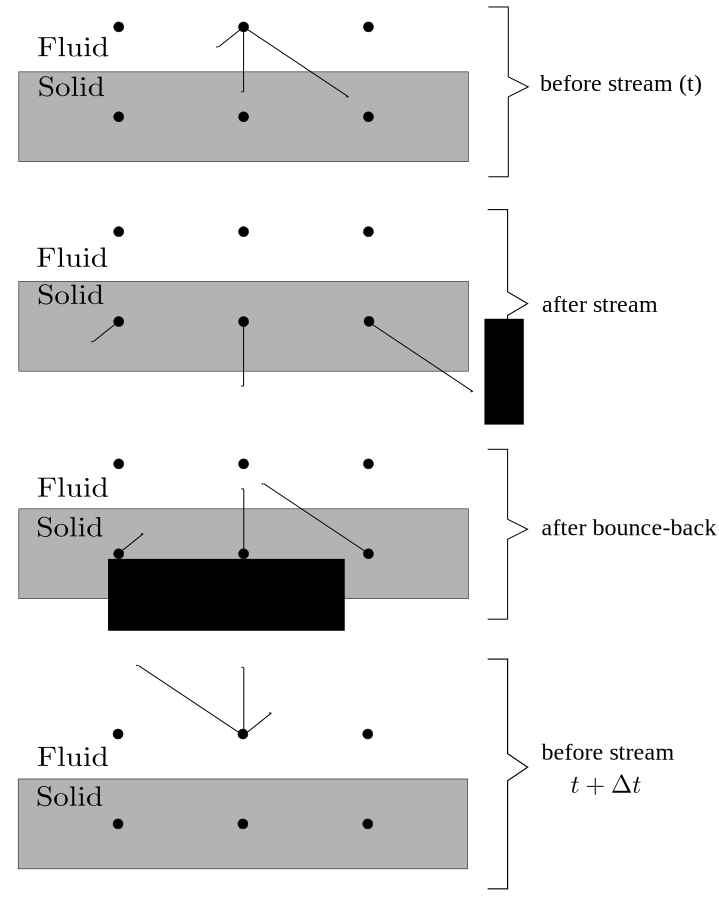
\includegraphics[width=0.5\textwidth]{bounce}
	\caption[Half-way bounce back algorithm for the \textit{D2Q9} model 
	]{Half-way 
	bounce back algorithm for the \textit{D2Q9} model adopted after 
	\citet{Sukop2006}.}
	\label{fig:bounce}
\end{figure}

\subsubsection*{Pressure and velocity boundary condition}

The pressure (Drichlet) boundary condition can be imposed in 
lattice Boltzmann by specifying a fluid density at the pressure 
boundary~\citep{Zou1997}. To impose a pressure boundary along 
the y-direction (for example, consider the left hand side inlet boundary 
in~\cref{fig:LBMcontour}), a 
density $\rho = \rho_{in}$ is specified from which the velocity is computed. 
The vertical component of the velocity on the boundary is set as zero, $u_y=0$. 
After streaming, $f_2, f_3, f_4, f_6,$ and $f_7$ are known, $u_x$ and $f_1, 
f_5, f_8$ are to be determined from~\cref{eq:lbm_macroscopic} as
%
\begin{align}
 f_1+f_5+f_8 & =  \rho_{in} - (f_0+f_2+f_3+f_4+f_6+f_7) 
 \label{eq:pressure1}\\
 f_1+f_5+f_8 & =  \rho_{in}u_x + (f_3+f_6+f_7) 
 \label{eq:pressure2} \\
 f_5 - f_8  & =  f_2 - f_4 +f_6 -f_7\,,
\end{align}
%
\noindent Consistency of~\cref{eq:pressure1,eq:pressure2} gives
%
\begin{equation}
u_x  = 1 - \frac{[f_0+f_2+f_4+2*(f_3+f_6+f_7)]}{\rho_{in}}\,.
\end{equation}

The bounce-back rule for the non-equilibrium part of the 
particle distribution normal to the inlet is used to find $f_1 
-f_1^{eq} = f_3 -f_3^{eq}$. The values of $f_5$ and $f_8$ can 
be obtained from $f_1$
%
\begin{align}
f_1 & = f_3 + \frac{2}{3} \rho_{in}u_x \nonumber \\ 
f_5 & = f_7 - \frac{1}{2}(f_2 - f_4) + \frac{1}{6}\rho_{in}u_x\nonumber \\ 
f_8 & = f_6 + \frac{1}{2}(f_2 - f_4) + \frac{1}{6}\rho_{in}u_x\,.
\end{align}

The corner node at inlet needs some special treatment. 
Considering the bottom node at inlet as an example, after 
streaming, $f_3, f_4, f_7$ are known; $\rho$ is 
defined, and $u_x = u_y = 0$. The particle distribution 
functions $f_1, f_2, f_5, f_6, $ and  $f_8$ are to be determined. The 
bounce-back rule for the non-equilibrium part of the particle 
distribution normal to the inlet and the boundary is used to 
find
%
\begin{align}
f_1 & = f_3 + (f_1^{eq}-f_3^{eq}) = f_3 \\
f_2 & = f_4 + (f_1^{eq}-f_3^{eq}) = f_4 \,.
\end{align}
%
\noindent Using these we can compute
%
\begin{gather}
f_5 = f_7 \\
f_6 = f_8 = \frac{1}{2}[\rho_{in} - (f_1 + f_2 + f_3 + f_4 + f_5 + f_6 + f_7 + 
f_8)]\,.
\end{gather}

Similar procedure can be applied to the top inlet node and the outlet 
nodes. Von Neumann boundary conditions constrain the flux at the boundaries. A 
velocity vector $u=\left[ u_0\mbox{ }v_0 \right]^T$ is specified, from which 
the density and pressure are computed based on the domain. The velocity 
boundary condition can be specified in a similar way~\citep{Zou1997}. The 
pressure and velocity boundary conditions contribute additional equation(s) 
to determine the unknown distribution functions. In the case of velocity 
boundary, the boundary condition equation is sufficient to determine the 
unknown distribution functions in the \textit{D2Q9} model, however the pressure 
boundary conditions 
require additional constitutive laws to determine the unknown distribution 
functions. 

%*******************************************************************************
\section{Validation of the lattice Boltzmann method}

To verify the incompressible LBM model implemented in the above section, 
numerical simulation of a transient development of steady state 
Poiseuille flow in a straight channel is performed. At $t=0$, the LBM water 
particles ($\rho=1000 kg/m^{3}$) are simulated to flow through a channel of 
width `H' (= 0.4 \si{\meter}) and simulation length `L' (2.5H) under constant 
body force. Periodic boundary conditions are applied at either end of the 
channel and the pressure gradient is set to zero, which simulates the condition 
of a continuous flow of fluid in a closed circular pipe. The length `L' has no 
effect on the simulation as no streamwise variation is detected in the 
solution. The parameters adopted in LBM simulation are presented 
in~\cref{table:lbm}. Sufficient time is allowed for the flow to travel beyond 
the required development length so that the flow is laminar~\citep{Durst2005}. 
The development length  $\mathrm{X}_{\mathrm{D}}$ required for a flow to be 
fully laminar is
%
\begin{equation}
X_{D}/H=[(0.619)^{1.6}+(0.0567 R_{e})^{1.6}]^{1/1.6} \,,
\end{equation}
%
\noindent where $R_{e}$ is the Reynolds number. The velocity profile at steady 
state is presented in~\cref{fig:LBMcontour}. A maximum 
horizontal velocity of 0.037863~\si{\meter\per\second} is observed along the 
center-line of the channel. The maximum horizontal velocity is compared with 
the closed-form based on the Haygen-Poiseuille flow equation for no-slip 
boundary condition~\citep{Willis2008}
%
\begin{equation}
	\mathit{U}_{\mathit{x}}=\frac{\Delta P}{2 \mu L} [\frac{H^{2}}{4}-y^{2}]\,,
\end{equation}
%
\noindent where $v_{x}$ is the horizontal velocity (m/s); $\Delta P$ is the 
pressure gradient, $\mu$ dynamic viscosity of the fluid. LBM predicts the 
maximum horizontal velocity within an error of 0.009~\%.

\begin{table}[tb]
\caption{LBM parameters used in simulating laminar flow through 
a circular pipe.}
\label{table:lbm}
\centering
\begin{tabular}{ll}
\toprule
\textbf{Parameter} & \textbf{Value} \\ \midrule
Density $\rho$ & 1000~\si{\kilogram\per\metre\cubed}\\ 
Relaxation parameter $\tau$ & 0.51\\ 
Kinematic viscosity  & $1 \times 10^{-6}$~\si{\metre\squared\per\second} \\
Grid resolution `h' & $1 \time 10^{-2} $~\si{\meter} \\
Number of steps & 50,000 \\
\midrule
Error in predicting horizontal velocity & 0.009 \% \\ \bottomrule
\end{tabular}
\end{table}

In order to further validate the accuracy of the lattice Boltzmann code, the 
transient development of the Poiseuille's flow is compared with the CFD 
simulation performed using ANSYS Fluent. Finite Volume Method is a 
common CFD technique, which involves solving the governing partial differential 
equation (Navier-Stokes) over the discretised control volume. This guarantees 
the conservation of fluxes over a particular control volume. The finite volume 
equations yield governing equations of the form
%
\begin{align}
\frac{\partial}{\partial t} \int\int\int  Q d\mathbf{V} + 
\int\int \mathit{F} d\mathbf{A} = 0\,,
\end{align}
%
where \textit{Q} is the vector of conserved variables, \textit{F} is the vector 
of fluxes in the Navier-Stokes equation, \textit{V} is the volume of control 
volume element, and \textit{A} is the surface area of the control volume 
element.

A 2D rectangular plane of length 1~\si{\meter} and height 0.04~\si{\meter} 
is discretised into 400 cells of size $1 \time 10^{-2} $~\si{\meter} 
(see~\cref{fig:CFDmesh}). A constant velocity is applied at the 
inlet. Water ($\rho = 998.2\mbox{ }kg/m^{3},\mbox{ } 
viscosity`\eta'=1 \times 10^{-3}\mbox{ } Ns/m^{2} $) is allowed to flow through 
the channel and it develops into a fully laminar flow. The least squares 
approach was adopted to solve the gradient, and a maximum of 100 
iteration steps were carried out until the solution converged. 

\begin{figure}[htbp]
	\centering
	\includegraphics[width=0.85\textwidth]{LBM_Poiseuille}
	\caption{Velocity profile: LBM Simulation of a laminar flow through a 
		channel.}
	\label{fig:LBMcontour}
\end{figure}
%
\begin{figure}[htbp]
	\centering
	\includegraphics[width=0.85\textwidth]{CFD_Mesh}
	\caption{Finite Volume mesh used in the CFD analysis of laminar flow 
	through a 
		channel.}
	\label{fig:CFDmesh}
\end{figure}
%
\begin{figure}[htbp]
	\centering
	\includegraphics[width=0.85\textwidth]{CFD_Poiseuille}
	\caption{Velocity profile: CFD analysis of laminar flow through a channel.}
	\label{fig:CFDcontour}
\end{figure}

The velocity profile obtained from the CFD simulation at cross-section `L/4' is 
shown in~\cref{fig:CFDcontour}.~\Cref{fig:Pois} compares the development of 
computed velocity profiles with the analytical solution. At normalised time $t 
= 1$, the flow approaches steady state. It can be observed that LBM has 
excellent agreement with CFD and the analytical solution at various stages of 
flow evolution.

\begin{figure}[tbhp]
	\centering
	\includegraphics[width=0.95\textwidth]{Poiseuille}
	\caption{Development of the Poiseuille velocity profile in time: comparison 
		between LBM simulation, CFD simulation and the analytical solution. 
		Time is 
		made dimensionless by $H/U_0$.}
	\label{fig:Pois}
\end{figure}

In order to study the capability of the lattice Boltzmann technique to simulate 
fluid--solid interaction, LB simulation of a fluid flow around a rectangular 
obstacle is compared with the CFD technique. A solid wall of height `H/2' is 
placed at length `L/4' in the channel. Bounce-back algorithm is employed to 
model the fluid-wall interaction in LBM. In the CFD model, the control volume 
is discretised into 10,000 cells. A constant velocity is applied in the inlet 
and the horizontal velocity profile is recorded. Both, CFD and LBM simulations 
were performed to study the influence of a solid wall on the fluid flow 
behaviour.

The horizontal velocity profile obtained after 50,000 LBM iterations is 
presented in~\cref{fig:LBMobstacle}. LBM is able to capture the velocity 
shedding around the edges of the wall. The velocity profile obtained from the 
CFD analysis is presented in~\cref{fig:CFDobstacle}. The horizontal velocity 
profile at `L/4' at $t=1$ is shown in~\cref{fig:Obstacle}. The maximum 
horizontal velocity from the CFD analysis is 0.3\% 
higher in comparison with the LBM simulation. The discrepancy in the horizontal 
velocity profile (\cref{fig:Obstacle}) can be attributed to the relaxation 
parameter used in the LBM, which is obtained by a trial and error procedure. 
The velocity profile obtained from the LBM simulation compares qualitatively 
with the FE analysis performed by~\citet{Zhong1991}. Thus, it can be concluded 
that the lattice Boltzmann method is a suitable form of numerical 
representation of the Navier-Stokes equation to model fluid -- solid 
interactions. 

\begin{figure}[!t]
\centering
\hspace{-13mm}\includegraphics[width=0.95\textwidth]{LBM_Obstacle}
\caption{LBM simulation of velocity profile for a laminar flow through a pipe 
with an obstacle at L/4.}
\label{fig:LBMobstacle}
\end{figure}

\begin{figure}[!ht]
\centering
\includegraphics[width=0.7\textwidth]{CFD_Obstacle}
\caption{CFD simulation of velocity contour for a laminar flow through a pipe 
with an obstacle at L/4.}
\label{fig:CFDobstacle}
\end{figure}

\begin{figure}[htbp]
\centering
\includegraphics[width=0.95\textwidth]{Obstacle}
\caption{LBM and CFD simulation of a flow around an obstacle.}
\label{fig:Obstacle}
\end{figure}


%**************************************************************************

\section{Turbulence in lattice Boltzmann method}

The above formulation of lattice Boltzmann has been successfully 
applied to many fluid flow problems, however it is restricted to flows with low 
Reynolds number. Modelling fluids with low viscosity like water and air 
remains a challenge, necessitating very small values of \textit{h}, and/or 
$\tau$ very close to 0.5~\citep{He1997}. The standard lattice Boltzmann can 
deal with laminar flows, while practical problems with small kinematic 
viscosity are often associated with flows having large Reynolds numbers, i.e. 
flows which are unsteady or turbulent in nature. The turbulent flows are 
characterised by the occurrence of eddies with multiple scales in space, time 
and energy.

The large eddy simulation (LES) is the most widely adopted approach to 
solve turbulent flow problems. It directly solves the large scale eddies, which 
carry the predominant portion of the energy, and the smaller eddies are 
modelled using a sub-grid approach. The separation of scales is achieved by 
filtering of the Navier-Stokes equations, from which the resolved scales are 
directly obtained. The unresolved scales are modelled by a one-parameter 
Smagorinski sub-grid methodology, which assumes that the Reynolds stress 
tensor is dependent only on the local strain rate~\citep{Smagorinsky1963}. It 
involves parametrising the turbulent energy dissipation in the flows, where the 
larger eddies extract energy from the mean flow and ultimately transfer some of 
it to the smaller eddies which, in turn, pass the energy to even smaller 
eddies, and so on up to the smallest scales. At the smallest scale, the eddies 
convert the kinetic energy into the internal energy of the fluid. At this 
scale, the viscous friction dominates the flow~\citep{Frisch1995}.

In the Smargonisky model, the turbulent viscosity $\nu$ is related to the 
strain 
rate $S_{ij}$ and a filtered length scale `h' as follows
%
\begin{align}
S_{ij} & = \frac{1}{2}(\partial_i u_j + \partial_j u_i) \\
\mathit{v}_{\mathit{t}} & = (\mathit{S}_{c}\mathit{h})^{2}\overline{S} \\
\overline{S} & =  
\sqrt{\sum\limits_{\mathit{i,j}}{\tilde{S}_{\mathit{i,j}}\tilde{S}_{\mathit{i,j}}}}\,,
\end{align}
%
\noindent where $\mathit{S}_{c}$ is the Smagorinski constant, which is close 
to 0.03~\citep{yu2005}. 
%
The effect of the unresolved scale motion is taken into account by introducing 
an effective collision relaxation time scale $\tau_{t}$, so that the total 
relaxation time $\tau_{*}$ is written as
%
\begin{equation}
\tau_{*}=\tau + \tau_{t}\,,
\end{equation} 
%
\noindent where $\tau$ and $\tau_{t}$ are respectively the standard relaxation 
times 
corresponding to the true fluid viscosity $\nu$ and the turbulence 
viscosity $\nu_{\mathit{t}}$, defined by a sub-grid turbulence model. 
The new viscosity $\nu_{*}$ corresponding to $\tau_{*}$ is defined as
%
\begin{align}
\nu_{*} & 
=\nu+\nu_{\mathit{t}} \nonumber \\
	& =\frac{1}{3}(\tau_{*}-\frac{1}{2})
\mathit{C}^{2} \Delta \mathit{t} 
=\frac{1}{3}(\tau+\tau_{t}-\frac{1}{2})\mathit{C}^{2} \Delta \mathit{t}  \\
\nu_{\mathit{t}} & =\frac{1}{3}\tau_{\mathit{t}}\mathit{C}^{2} \Delta 
\textit{t} \,.
\end{align} 

The Smagorinski model is easy to implement and the lattice Boltzmann 
formulation remains unchanged, except for the use of a new turbulence-related 
viscosity $\tau_{*}$. The component $s_1$ of the collision matrix becomes $s_1 
= \frac{1}{\tau+\tau_t}$.

The effectiveness of LBM-LES model in simulating unsteady flows is verified by 
modelling the K\'{a}rm\'{a}n vortex street. In fluid dynamics, a K\'{a}rm\'{a}n 
vortex street is a repeating pattern of vortices caused by unsteady separation 
of fluid flow around circular obstacles. A vortex street will only be observed 
above a limiting value of Reynolds number of 90. The Reynolds number 
is computed based on the cylinder diameter `D' and the mean flow velocity $U$ 
of the parabolic inflow profile
%
\begin{equation}
\label{eq:reynolds}
Re=\frac{UD}{\nu}\,.
\end{equation}

LBM particles are simulated to flow through a 2D rectangular channel with an 
aspect ratio `L/H' of 2.5. A cylinder of diameter `d' $=0.27H$ is placed at 
H/2. The pressure gradient at the inlet and the outlet is varied to create 
flows with different mean velocities. Numerical simulations of vortex 
shedding behind a circular obstacle are carried out for three different fluid 
flow regimes (Reynolds number of 55, 75, and 112). The fully developed fluid 
flows for different Reynolds numbers are shown in~\cref{fig:karman}. It can be 
observed from~\cref{fig:karman} that the von K\'{a}rm\'{a}n vortex street can 
only be observed at high a Reynolds number of 112 (Re > 90), which shows the 
ability of the LBM turbulence model to capture instabilities in fluid flow.
%
\begin{figure}[htbp]
	\centering
	\includegraphics[width=0.95\textwidth]{karman}
	\caption{K\'{a}rm\'{a}n vortex street}
	\label{fig:karman}
\end{figure}

One important quantity taken into account in the present analysis is the 
Strouhal number St, a dimensionless number describing oscillating unsteady 
flow dynamics. The Strouhal number is computed from the cylinder diameter D, 
the measured frequency of the vortex shedding f, and the maximum velocity 
$U_{max}$ at the inflow plane
%
\begin{equation}
St=\frac{fD}{U_{max}}\,.
\end{equation}

\noindent The characteristic frequency $f$ is determined by a spectral 
analysis (Fast Fourier Transform - FFT) of time series of the fluid pressure. 
\Cref{table:strouhal} shows that the Strouhal numbers computed from LBM 
simulations have a very good agreement with FVM results obtained 
by~\citet{Breuer2000}. This shows the ability of LBM-LES in capturing unsteady 
flow dynamics.


\begin{table}[tbhp]
	\caption{Computed Strouhal number for fluid flows with different Reynolds 
	number}
	\label{table:strouhal}
	\centering
	\begin{tabular}{l c c}
		\toprule
		Reynolds number & \multicolumn{2}{c}{Strouhal number} \\
		\cmidrule{2-3}
		& LBM & FVM \\
		\midrule
		55		& 0.117	 &	0.117 \\
		75		& 0.128	 &	0.129 \\
		112		& 0.141  &	0.141 \\
		\bottomrule
		\multicolumn{3}{l}{\footnotesize{\textsuperscript{*}~FVM results are 
		from~\citet{Breuer2000}}}
	\end{tabular}
\end{table}



%************************************************************************* %

\section{Coupled LBM and DEM for fluid-grain interactions}

Modelling fluid--grain interactions in submarine landslides requires the 
ability to simulate the interactions at the dynamic fluid -- solid boundaries. 
In principle, the conventional FE and FVM based approaches for solving the 
Navier-Stokes equations with moving boundaries and/or structural 
interaction~\citep{Bathe2004} can be applied to particle fluid interaction 
problems. The common feature of these approaches is to model the interaction 
between the fluid and the solid to a high degree of accuracy. However, the main 
computational challenge is the need to continuously generate new geometrically 
adapted meshes to circumvent severe mesh distortion, which is computationally 
very intensive~\citep{Han2007a}. 

The lattice Boltzmann approach has the advantage of accommodating large 
particle sizes and the interaction between the fluid and the moving grains 
can be modelled through relatively simple fluid - grain interface treatments. 
Further, employing DEM to account for the grain/grain interaction naturally 
leads to a combined LB -- DEM solution procedure. The Eulerian nature 
of the lattice Boltzmann formulation, together with the common explicit time 
step scheme of both LBM and DEM makes this coupling strategy an efficient 
numerical procedure for the simulation of fluid -- grain systems. 

LBM -- DEM technique is a powerful predictive tool for gaining insights into 
many fundamental physical phenomena in fluid-solid systems. 
Such a coupled methodology was first proposed by~\citep{Cook2004} for 
simulating fluid-grain systems dominated by fluid-grain and grain-grain 
interactions. To capture the actual physical behaviour of the fluid-grain 
system, it is essential to model the boundary condition between the fluid and 
the grain as a non-slip boundary condition, i.e. the fluid velocity near the 
grain should be similar to the velocity of the grain boundary. The soil grains 
in the fluid domain are represented by lattice nodes. The discrete nature of 
the lattice will result in stepwise representations of the surfaces, which are 
otherwise circular, this is  neither accurate nor smooth, unless sufficiently 
small lattice spacing is adopted. 

%*******************************************************************************%

\subsubsection*{Modified bounce back rule}

To accommodate the movement of solid particles in the commonly adopted 
bounce-back rule (see \cref{bounce}),~\citet{Ladd1994} modified the `no-slip' 
rule for a given boundary link \textit{i} to be
%
\begin{equation}
\mathit{f_i}(\mathbf{x}, t + \Delta t)=\mathit{f_i}(\mathbf{x}, t_{+}) - 
\alpha_{\mathit{i}}\mathbf{\mathit{e}_i}.\mathbf{\mathit{v}}_{b} \qquad 
(\alpha_{i}=6\mathit{w_i}\rho/\mathit{C}_{\mathit{s}}^{2})\,,
\end{equation}
%
\noindent where $\mathit{f_i}(\mathbf{x}, t_{+})$ is the post collision 
distribution at the fluid or solid boundary node \textbf{x}, and 
$\mathit{v}_{b}$ is the velocity at the nominal boundary point at the middle of 
the boundary link \textit{i}
%
\begin{equation}
\mathbf{v}_{b}=\mathbf{v}_{c}+\omega \times 
(\mathbf{x}+\mathbf{\mathit{e}_i}\Delta t /2 - \mathbf{x}_{c})\,,
\end{equation}
%
\noindent in which $\mathbf{\mathit{v}}_{c}$ and $\omega$ are the translational 
and angular velocities at the mass centre of the solid particle, respectively. 
$\mathbf{x}_{c}$ and $\mathbf{x}+\mathbf{\mathit{e}_i}\Delta t /2$ are the 
coordinates of the centre and the nominal boundary point,  respectively. The 
impact force on the soil grain from the link is defined as
%
\begin{equation}
\mathbf{F_i}=2[\mathit{f_i} (\mathbf{x}, t_{+}) 
-\alpha_{\mathit{i}}\mathbf{\mathit{e}_i}.\mathbf{v}_{b}]/ \Delta t \,.
\end{equation} 
%
The corresponding torque $\mathbf{T}_{\mathit{i}}$, produced by the force with 
respect to the centre of the particle is computed as
%
\begin{equation}
\mathbf{T}_{\mathit{i}}=\mathbf{r}_{c} \times \mathit{F_i} 
(\mathbf{r}_{c}=\mathbf{x}+\mathbf{e}_{\mathit{i}} \Delta t /2 - \mathbf{x}_{c})
\,.
\end{equation}
%
Then the total hydrodynamic force and torque exerted on the particle can be 
calculated by summing up the forces and torques from all the related boundary 
links
%
\begin{equation}
\begin{aligned}
\mathbf{F} &= \sum\limits_{\mathit{i}}{\mathbf{F}_{\mathit{i}}} \\
\mathbf{T} &= \sum\limits_{\mathit{i}}{\mathbf{T}_{\mathit{i}}} \,.
\end{aligned}
\end{equation}

\citet{Ladd2001} described a methodology that minimises the oscillations 
resulting from soil grains crossing lattices at a very high speed. The 
methodology involves combining several extensions for the fluid simulation like 
the treatment of moving curved boundaries with the scheme of~\citet{Yu2003} and 
a fluid/grain force interaction method with the momentum exchange method  
of~\citet{Ladd2001}. The simulation of the moving curved grain surfaces results 
in the intersection of links between two nodes at arbitrary 
distances~\citep{Iglberger2008}. These distance values are called as delta 
values
%
\begin{equation}
\delta = \frac{\mbox{Distance between fluid node and soil
surface}}{\mbox{Distance between fluid node and soil node}} \in [0,1] \,.
\end{equation} 
%
For each pair of a fluid and grain node, a delta value has to be 
calculated. Delta values of zero are not possible as the nodes on the surface 
are considered as solid nodes. The algorithm for computation of the $\delta$ 
value is presented in~\citet{Iglberger2008}.~\Cref{fig:bouncemod} shows the 
three possible situations for delta values between 0 and 1. The 
fluid particles in LBM are always considered to be moving at the rate of one 
lattice per time step $(\delta \mathbf{x}/ \delta \mathbf{t})$, for delta 
values smaller than 0.5. For $\delta$ values larger than 0.5, the fluid 
particles would come to rest at an intermediate node $\mathbf{x}_{\mathit{i}}$. 
In order to calculate the reflected distribution function in node 
$\mathbf{x}_{\mathit{f}}$, an interpolation scheme has to be applied. The 
linear interpolation scheme of~\citet{Yu2003} is used in the present study, 
which uses a single equation, irrespective of the value of $\delta$ being 
smaller or larger than 0.5, to the reflected distribution function that is 
computed as
%
\begin{align}
 \nonumber
\mathit{\mathit{f}}_{\overline{\alpha}}(\mathbf{x}_{\mathit{f}},t + \delta t) = 
& \frac{1}{1 + \delta} \cdot [(1-\delta)\cdot 
\mathit{\mathit{f}}_{\alpha}(\mathbf{x}_{\mathit{f}},t + \delta t) + \delta 
\cdot \mathit{\mathit{f}}_{\alpha}(\mathbf{x}_{\mathit{b}},t + \delta t)  \\
& + \delta \cdot 
\mathit{\mathit{f}}_{\overline{\alpha}}(\mathbf{x}_{\mathit{f2}},t + \delta t) 
-2\mathit{w}_{\mathit{a}}\rho_{\mathit{w}}\frac{3}{\mathit{c}^{2}}
	\mathbf{\mathit{e}}_{\mathit{a}}\cdot
 \mathbf{u}_{\mathit{w}}]\,,
\end{align}
%
where $\mathit{w}_{\alpha}$ is the weighting factor, $\rho_{\mathit{w}}$ is the 
fluid density in node $\mathbf{x}_{\mathit{f}}$, and $ \mathbf{u}_{\mathit{w}}  
$ is the velocity at the bounce-back wall. In order to couple the 
fluid-grain interaction, the LBM approach is extended by adopting a force 
integration scheme, to calculate the fluid force acting on the grain surface, 
and the momentum exchanged method described earlier. The physical force acting 
on grain agglomerates is calculated as the sum over all fluid/grain node 
pairs, resulting in
%
\begin{equation}
\mathit{F} = 
\sum\limits_{\mathbf{x}_{b}}\sum\limits_{\alpha=1}^{19}{\mathbf{e}_{\alpha}
	[\mathit{f}_{\alpha}(\mathbf{x}_{b},t)
		+\mathit{f}_{\overline{\alpha}}(\mathbf{x}_{f},t)]
 				\delta \mathbf{x} / \delta t}\,.
\end{equation}
%
After the force calculations, the coupled rigid body physics can be simulated 
in order to move the grains / grain-agglomerates according to the applied 
forces. The total hydrodynamic forces and torque exerted on a grain can be 
computed as ~\citep{Cook2004, Noble1998}
%
\begin{align}
\mathbf{F}_{f} & = \mathit{Ch}[\sum\limits_{\mathit{n}}{(\beta_{\mathit{n}} 
\sum\limits_{\mathit{i}}{\mathit{f_i}^{\mathit{ m}}\mathbf{\mathit{e}_i}}})] \\ 
\mathbf{T}_{f} & = 
\mathit{Ch}[\sum\limits_{\mathit{n}}{(\mathbf{x}_{\mathit{n}}-\mathbf{x}_{\mathit{c}})
 \times (\beta_{\mathit{n}} \sum\limits_{\mathit{i}}{\mathit{f_i}^{\mathit{ 
m}}\mathbf{\mathit{e}_i}})}]\,.
\end{align}
%
The summation is over all lattice nodes covered by the soil grain, and 
$\mathbf{x}_{\mathit{n}}$ represents the coordinate of the lattice node 
\textit{n}.
%
\begin{figure}[htbp]
\centering
\includegraphics[height=0.9\textheight]{bouncemod}
\caption{Bounce back boundaries for different values of $\delta$}
\label{fig:bouncemod}
\end{figure}

When grains are not in direct contact among themselves, but are driven by 
the fluid flow and body force, i.e. gravity, their motion can be determined by 
Newton's equation of motion
%
\begin{align}
\mathit{m}\mathbf{ a} & = \mathbf{F}_{f} + \mathit{m }\mathbf{g} \\
\mathit{J } \ddot{\theta} & = \mathbf{T}_{f} \,,
\end{align}
%
\noindent where \textit{m} and \textit{J} are respectively the mass and the 
moment of inertia of a grain, $\ddot{\theta}$ is the 
angular acceleration, \textbf{g} is the gravitational acceleration,
$\mathbf{F}_{f}$ and $\mathbf{T}_{f}$ are respectively the hydrodynamic forces 
and torque. The equation can be solved numerically by an explicit numerical 
integration, such as the central difference scheme. 

The interaction between the soil grains, and the soil grains with the walls are 
modelled using the DEM technique. To solve the coupled DEM--LBM formulation, 
the 
hydrodynamic force exerted on soil grains and the static buoyancy force are 
considered by reducing the gravitational acceleration to $(1- 
\rho/rho_{s})\mathbf{g}$, where $\rho_{s}$ is the density of the grains. When 
taking into account all forces acting on an element, the dynamic equations of 
DEM can be expressed as
%
\begin{equation}
\label{eq:mde}
\mathit{m}\mathbf{a} +\mathit{c}\mathbf{v} = \mathbf{F}_{c} + \mathbf{F}_{f} 
+\mathit{m}\mathbf{g} \,,
\end{equation} 
%
\noindent where $\mathbf{F}_{c}$ denotes the total contact forces from other 
elements and/or the walls, and \textit{c} is a damping coefficient. The term 
\textit{c\textbf{v}} represents a viscous force that accounts for the effect of 
all possible dissipation forces in the system including energy lost during the 
collision between grains. Considering a linear contact model
%
\begin{equation}
\mathbf{F}_{c}=\mathit{k}_{\mathit{n}} \delta \,,
\end{equation}
%
\noindent where $\mathit{k}_{\mathit{n}}$ is the normal stiffness and $\delta$ 
is the overlap, the critical time step associated with the explicit integration 
is determined as~\citep{He1997}
%
\begin{equation}
\Delta t_{\mathit{cr}}= 2(\sqrt{1 + \xi^{2}}-\xi) / \omega \,,
\end{equation}
%
\noindent where $\omega = \sqrt{\mathit{k}_{\mathit{n}}/\mathit{m}}$ is the 
local contact natural frequency and $\xi = \mathit{c}/2\mathit{m}\omega$ is the 
critical damping ratio. The actual time step used for the integration of the 
Discrete Element equations is
%
\begin{equation}
\Delta \mathit{t}_{D}=\lambda \Delta \mathit{t}_{cr} \,.
\end{equation}
%
The time step factor $\lambda$ is chosen to be around 0.1 to ensure both 
stability and accuracy~\citep{He1997}.

When combining the Discrete Element modelling of the grain interactions with 
the LB formulation, an issue arises. There are now two time steps: $\Delta t$ 
for the fluid flow and $\Delta t_{D}$ for the particles. Since $\Delta t_{D}$ 
is normally smaller than $\Delta t$, $\Delta t_{D}$ is slightly reduced to a 
new value $\Delta t_{s}$ so that $\Delta t$ and $\Delta t_{s}$ have an integer 
ratio $\mathit{n}_{\mathit{s}}$
%
\begin{align}
\Delta t_{s}=\frac{\Delta t}{\mathit{n}_{s}} \qquad(\mathit{n}_{s}=[\Delta t/ 
\Delta t_{D}]+1) \,.
\end{align} 
%
This results in a sub-cycling time integration for the Discrete 
Element part. At every step of the fluid computation, $\mathit{n}_{s}$ 
sub-steps of integration are performed for the Discrete Element 
Method~\eqref{eq:mde} using the time step $\Delta t_{s}$. The hydrodynamic 
force $\mathbf{F}_{f}$ is unchanged during the sub-cycling. 

\subsection{Draft, kiss and tumbling: Sedimentation of two grains}

In multiphase flows, fundamental mechanisms of fluid -- grain and grain – grain 
interactions are very important for accurately predicting the flow behaviours. 
The sedimentation of two circular grains in a viscous fluid serves as the 
simplest problem to study these two types of interactions, and many 
experimental and numerical studies have been carried out to investigate this 
behaviour~\citep{Wang2014,Komiwes2005}.~\citet{Fortes1987} observed 
experimentally that in the sedimentation of two grains under gravity in a 
Newtonian fluid, the two grains would undergo the draft, kiss and tumbling 
(DKT) phenomenon.

The \emph{draft}: grain 2 is first placed within the hydrodynamic drag above 
grain 1. As the hydrodynamic drag of grain 1 is a depression zone, 
grain 2 is attracted inside. The \emph{kiss}: grain 2 increases its 
vertical velocity until it touches grain 1. The horizontal velocity of 
grain 1 increases and its vertical velocity decreases below that of 
grain 2. \emph{Tumbling}: grain 2 having the same horizontal velocity and 
higher vertical velocity than grain 1, overtakes grain 1.
%

LBM-DEM simulation of two grains under gravity in a viscous Newtonian fluid 
reproduces the draft, kiss and tumble effect (see~\cref{fig:kissing}). They 
are in agreement with the experimental description of the DKT effect. For 
better understanding of the DKT effect, the time history of three distances 
between the grains (normalised to the diameter of the grain D) are tracked 
i.e., the difference in the transverse coordinates $\delta_x/D$ and 
longitudinal coordinates $\delta_y/D$ of the two grain centres, and the gap 
between the two surfaces $\delta = \sqrt{{\delta_x}^2+{\delta_y}^2} - 1 $ 
(see~\cref{fig:kissdelta}). 

As shown in~\cref{fig:kissing}, grain 1 trails grain 2. As grain 2 approaches 
the depression zone, corresponding to negative fluid pressure behind grain 1, 
the velocity of the trailing grain increases as the grains approach closer, 
this is in agreement with the experimental description of the draft. Grain 2 
increases its vertical velocity more than grain 1 until it touches grain 1. The 
kiss happens at a normalised time ($t/\sqrt{(D/g)}$)  = 25. At this stage, the 
gap $\delta$ between the grains is zero, but the actual gap is about one 
lattice spacing for the LBM collision model. After this time, the vertical 
velocity of grain 1 decreases and its horizontal velocity increases as the 
grains tumble. At this stage, the grains still remain in contact, i.e., the gap 
remains unchanged $\delta=0$. Subsequently, the two grains separate and move 
away from each other.~\Cref{fig:kissvelocity} shows that the terminal 
velocities of the two grains are in good agreement with the terminal velocity 
of a single grain found by an independent simulation and calculated using the 
empirical Schiller and Nauman formula~\citep{Komiwes2005}.

\begin{figure}[tbhp]
\centering
\includegraphics[height=0.9\textheight]{kissing}
\caption{Time series of draft, kiss and tumble of two grains during 
sedimentation in a viscous fluid.}
\label{fig:kissing}
\end{figure}

\begin{figure}[tbhp]
	\centering
	\begin{subfigure}[b]{0.475\textwidth}
		\includegraphics[width=\textwidth]{Kissing_xy}
		\caption{transverse and longitudinal position}
		\label{fig:kissxy}
	\end{subfigure}
	\begin{subfigure}[b]{0.475\textwidth}
		\includegraphics[width=\textwidth]{Kissing_velocity}
		\caption{normalised velocity}
		\label{fig:kissvelocity}
	\end{subfigure}\\
	\begin{subfigure}[b]{0.475\textwidth}
		\includegraphics[width=\textwidth]{Kissing_delta}
		\caption{distance between grains}
		\label{fig:kissdelta}
	\end{subfigure}
	\caption{Time history of two circular grains during sedimentation.}
	\label{fig:kiss}
\end{figure}

\section{GP-GPU Implementation}

Graphics Processing Unit (GPU) is a massively multi-threaded architecture that 
is widely used for graphical and now non-graphical computations. Today's GPUs 
are general purpose processors with support for an accessible programming 
interface. The main advantage of GPUs is their ability to perform significantly 
more floating point operations (FLOPs) per unit time than a CPU. General 
Purpose computations on GPUs (GPGPUs) often achieve speedups of orders of 
magnitude in comparison with optimised CPU implementations. 

A GPU consists of several \emph{Streaming Multiprocessors} (SMs). Each SM 
contains 32 CUDA processors. Each CUDA processor has a fully pipelined integer 
arithmetic logic unit (ALU) and a floating point unit (FPU). The FPU complies 
with the IEEE 754-2008 industry standard for floating-point arithmetic, capable 
of double precision computations. The SM schedules work in groups of 32 threads 
called warps. Each SM features two warp schedulers and two instruction dispatch 
units, allowing two warps to be issued and executed concurrently. Each thread 
has access to both L1 and L2 caches, which improves the performance for 
programs with random memory access.

The occupancy rate of the SPs, i.e. the ratio between the 
number of threads run and the maximum number of executable threads, is an 
important aspect to take into consideration for the optimisation of a CUDA 
kernel. Even though a block may only be run on a single SM, it is possible to 
execute several blocks concurrently on the same SM. Hence, tuning the execution 
grid layout allows one to increase the occupancy rate. Nevertheless, reaching 
the maximum occupancy is usually not possible, as the threads executed in 
parallel on one SM have to share the available registers~\citep{Obrecht2011}.

Many-core processors are promising platforms for intrinsically parallel 
algorithms such as the lattice Boltzmann method. Since the global memory 
for GPU devices shows high latency and LBM is data intensive, the
memory access pattern is an important issue for achieving good performances. 
Whenever possible, global memory loads and stores should be coalescent and 
aligned, but the propagation phase in LBM can lead to frequent misaligned 
memory accesses. Also, the data transfer between the host and the device is 
very expensive. In the present study, the LBM implementation follows carefully 
chosen data transfer schemes in global memory.

There are three ways to accelerate GPGPU applications: (a) Using `drop-in' 
libraries, (b) using directives by exposing parallelism, and (c) using 
dedicated GPGPU programming languages. OpenACC (Open Accelerators) is an open 
GPU directives programming standard for parallel computing on heterogeneous 
CPU/GPU systems. Unlike conventional GPU programming languages, such as CUDA, 
OpenACC uses directives to specify parallel regions in the code and performance 
tuning works on exposing parallelism. OpenACC targets a host-directed execution 
model where the sequential code runs on a conventional processor and 
computationally intensive parallel pieces of code (kernels) run on an 
accelerator such as a GPU (see~\cref{fig:GPUConcept}). 

The original GPGPU LBM -- DEM code was implemented in C using OpenACC API v1.0, 
which was released in November 2011. The current implementation in C++ uses 
OpenACC API v2.0a~\citep{OpenACCmembers2013} and has two compute 
constructs, the kernels construct and the parallel construct. LBM -- DEM 
implementation predominantly uses the OpenACC gang and vector parallelism. The 
LBM -- DEM code runs sequential and computationally less intensive 
functions on the CPU, OpenMP multi-threading is used when possible. 
Computationally intensive functions are converted to a target accelerator 
specific GPU parallel code. Schematics of a heterogeneous CPU/GPU system is 
shown in~\cref{fig:GPUConcept}.

\begin{figure}[tbhp]
	\centering
	\includegraphics[width=0.92\textwidth]{GPU_Concept}
	\caption{Schematics of a heterogeneous CPU/GPU system.}
	\label{fig:GPUConcept}
\end{figure}

OpenACC offers kernel and parallel constructs to parallelise algorithms on CUDA 
kernels. The loop nests in a kernel construct are converted by the compiler 
into parallel kernels that run efficiently on a GPU. There are three steps to 
this process. The first is to identify the loops that can be executed 
in parallel. The second is to map that abstract loop parallelism onto a 
concrete hardware parallelism. In OpenACC terms, gang parallelism maps to 
grid-level parallelism (equivalent to a CUDA blockIdx), and vector parallelism 
maps to thread-level parallelism (equivalent to a CUDA threadIdx). The compiler 
normally maps a single loop across multiple levels of parallelism using 
strip-mining. Finally, in step three the compiler generates and optimizes the 
actual code to implement the selected parallelism mapping.

An OpenACC parallel construct creates a number of parallel threads that 
immediately begin executing the body of the parallel construct redundantly. 
When a thread reaches a work-sharing loop, that thread will execute some subset 
of the loop iterations, depending on the scheduling policy as specified by the 
program or at the runtime. The code generation and optimization for a parallel 
construct is essentially the same as for the kernel construct. A key 
difference is that unlike a kernel construct, the entire parallel construct 
becomes a single target parallel operation, aka a single CUDA kernel. Both 
constructs allow for automatic vectorization within the loops~\citep{Wolfe2012}.

An excerpt from the LBM-DEM code showing the OpenACC GPU implementation of the 
hydrodynamic force compuration is presented in Listing~\ref{lst:GPU}. The 
kernels loop construct tells the compiler to map the body of the following loop 
into an accelerator kernel. The GPU implementation uses a two-dimensional grid 
splitting the iterations across both the vector and gang modes. The kernel is 
mapped to a vector mode mapped (aligned with CUDA threadidx\%x) with a vector 
length (thread block size) of 128. The kernel is also mapped to gang 
parallelism, aligned to CUDA blockidx\%x, to avoid partition camping by mapping 
the stride-1 loop to the x dimension. The compiler strip-mines the loop into 
chunks of 256 iterations, mapping the 256 iterations of a chunk in vector mode 
across the threads of a CUDA thread block, and maps the n/256 chunks in gang 
mode across the thread blocks of the CUDA grid. The consecutive iterations (i 
and i+1), which refer to contiguous array elements (fhf[i] and fhf[i+1]), are 
mapped to adjacent CUDA threads in the same thread block, to optimize for 
coalesced memory accesses. 



\begin{lstlisting}[label=lst:GPU,caption= OpenACC GPU implementation of the 
hydrodynamic force computation.,style=customcpp]
//OpenACC Kernels copy data between the host and the device
#pragma acc kernels 
copyout(fhf1[0:nbgrains], fhf2[0:nbgrains], fhf3[0:nbgrains]) 
copyin(obst[0:][0:], g[0:nbgrains], ey[0:], f[0:][0:][0:], ex[0:])
//Create individual threads for each DEM grain
#pragma acc parallel for
for (i=0; i<nbgrains;i++) {
  // Reset hydrodynamic forces to zero at the start of time step
  fhf1[i]=fhf2[i]=fhf3[i]=0.;
  // Iterate through all lattice nodes
  for (y=0; y<ly;y++) {
    for (x=0; x<lx;x++) {
      if(obst[x][y]==i) {
        // generate code to execute the iterations in parallel with
        // no synchronization
        #pragma acc for independent
        for (iLB=1; iLB<Q; iLB++) {
          next_x=x+ex[iLB];
          next_y=y+ey[iLB];
          if(iLB<=half) halfq=half;
          else halfq= $-$half;
          if(obst[next_x][next_y]!=i) {
            fnx=(f[x][y][iLB+halfq]+f[next_x][next_y][iLB])*ex[iLB+halfq];
            fny=(f[x][y][iLB+halfq]+f[next_x][next_y][iLB])*ey[iLB+halfq];
            fhf1[i]=fhf1[i]+fnx;
            fhf2[i]=fhf2[i]+fny;
            fhf3[i]=fhf3[i]$-$fnx*(y$-$(g[i].x2$-$wall_bottom_y)/dx) 
                    +fny*(x$-$(g[i].x1$-$wall_left_x)/dx);
          }			
        }
      }
    }
  }
}
\end{lstlisting}

Memory transaction optimisation is more important than computation
optimisation. Registers do not give rise to any specific problem apart from 
their limited amount. Global memory, being the only one accessible by both the 
CPU and the GPU, is the critical path as it suffers from high latency. However, 
this latency is mostly hidden by the scheduler which stalls inactive warps 
until data are available. For data intensive LBM, this aspect is generally the 
limiting factor~\citep{Obrecht2011}. To optimise the global memory 
transactions, the memory access is coalesced and aligned, as explained above. 
The memory transactions between the host and the target through a PCI bus are 
kept to a minimum.

A two-dimensional fluid -- grain system, which consists of 7.2 million LBM 
nodes and 2500 DEM grains is used to demonstrate the ability of the GPGPU LBM 
-- DEM code. The wall time required to compute 100 iterations of the given LBM 
-- DEM  problem is compared for executions running on a single CPU thread, 
multi-threaded CPU (using OpenMP) and the GPGPU implementations 
(see~\cref{table:GPU}). The speed-up of parallel implementations are measured 
against the single CPU thread execution time. OpenMP parallelised 
multi-threaded CPU execution running on 12 cores achieved a speed-up of 13.5x 
in comparison to a serial implementation. GPGPU implementation using OpenACC 
delivered an impressive 126x speed-up in comparison to a single thread CPU 
execution and about 10 times quicker than a CPU parallel code. In other words, 
a simulation that would have ordinarily taken 126 days to compute, could now be 
finished in a day using a GPU.

\begin{table}[tbhp]
	\caption{GPU vs CPU parallelisation}
	\label{table:GPU}
	\centering
	\begin{tabular}{l l l}
		\toprule
		Execution & Computational Time (s) &  Speedup \\
		\midrule
		CPU 1 OpenMP thread		& 2016	 & -- \\
		CPU 2 OpenMP threads	& 1035	 & 1.5 x \\
		CPU 4 OpenMP threads	& 660 	 & 3.0 x \\
		CPU 12 OpenMP threads	& 150	 & 13.5 x\\
		GPU OpenACC				& 16	 & 126.0 x \\
		\bottomrule
		\multicolumn{3}{l}{\footnotesize{\textsuperscript{\#}}~Wall time 
		for 100 iteration for 7.2 Million LBM nodes and 2500 DEM grains.} \\
		\multicolumn{3}{l}{\footnotesize{\textsuperscript{*}~CPU OpenMP threads 
		- 6 core Intel Xeon $\mathrm{@}$ 3.3GHz}} \\
		\multicolumn{3}{l}{\footnotesize{\textsuperscript{\dag}~GPU threads - 
		GeForce GTX 580 - 512 CUDA cores}}
	\end{tabular}
\end{table}

Scalability is an important criterion when developing high-performance 
computing codes. Scalability in GPUs is measured in terms of SM utilisation. It 
is important to distribute sufficient work to all SMs such that on every cycle 
the warp scheduler has at least one warp eligible to issue instructions. In 
general, sufficient warps on each SM should be available to hide instruction 
and memory latency and to provide a variety of instruction types to 
fill the execution pipeline.~\Cref{fig:GPUSpeed} shows the scalability of 
GP-GPU implementation as the LBM domain size is increased from 500,000 to 9 
million nodes. With increase in LBM nodes the computation time increases 
linearly with a slope of about 2, which shows that the LBM--DEM implementation 
algorithm scales with the domain size.

\begin{figure}[tbhp]
	\centering
	\includegraphics[width=0.85\textwidth]{GPU_Speedup}
	\caption{GPU scalability with increase in LBM nodes}
	\label{fig:GPUSpeed}
\end{figure}